% SPDX-License-Identifier: CC-BY-4.0
% Figure 1 - the heralded single-photon storage experiment (simplified).
% Original illustration based on the setup described in Buser et al. 2022,
% arXiv:2204.12389, Sections III-V and Fig. 2. Not a copy of any published figure.
\documentclass[tikz, border=0pt]{standalone}
% SPDX-License-Identifier: CC-BY-4.0
% styles.tex - shared typography, colours and TikZ styles for all HeraldRT figures.
%
% Conventions used in every figure
%   optical path        red, solid, 1.2pt, open arrow head
%   electrical event    blue, solid, 0.9pt (detector pulses, herald)
%   control output      green, dashed, 0.9pt (electronics -> actuators)
%   host / config       grey, dotted
%   implemented block   solid outline     proposed block   dashed grey outline
%   asynchronous domain light amber fill  synchronous domain light blue fill

\usepackage{fontspec}
\usepackage{unicode-math}
\setmainfont{FiraSans}[
  Extension = .otf, UprightFont = *-Book, BoldFont = *-SemiBold,
  ItalicFont = *-BookItalic, BoldItalicFont = *-SemiBoldItalic]
\setsansfont{FiraSans}[
  Extension = .otf, UprightFont = *-Book, BoldFont = *-SemiBold,
  ItalicFont = *-BookItalic, BoldItalicFont = *-SemiBoldItalic]
\setmathfont{FiraMath-Regular.otf}
\setmonofont{FiraMono}[Extension = .otf, UprightFont = *-Regular, BoldFont = *-Medium,
  Scale = 0.92]
\renewcommand{\familydefault}{\sfdefault}

\usepackage[detect-all]{siunitx}
\sisetup{range-phrase = --, range-units = single, per-mode = symbol}

\usepackage{tikz}
\usetikzlibrary{arrows.meta, positioning, calc, fit, backgrounds,
  decorations.pathmorphing, decorations.markings, shapes.geometric, shapes.misc}

% layer for domain shading: above the white page, below blocks and wires
\pgfdeclarelayer{board}
\pgfdeclarelayer{domains}
\pgfsetlayers{background, board, domains, main}

% reproducible PDF (no creation date / ID differences between builds)
\pdfvariable suppressoptionalinfo 1023

% ------------------------------------------------------------------ colours
\definecolor{ink}{HTML}{1B2631}
\definecolor{optical}{HTML}{B03A2E}
\definecolor{opticallight}{HTML}{F2D7D5}
\definecolor{pumpviolet}{HTML}{6C3483}
\definecolor{elec}{HTML}{1F4E79}
\definecolor{ctrl}{HTML}{1E7B4A}
\definecolor{host}{HTML}{6E7B85}
\definecolor{asyncfill}{HTML}{FDF2E3}
\definecolor{asyncline}{HTML}{C07A1E}
\definecolor{syncfill}{HTML}{EAF2FA}
\definecolor{syncline}{HTML}{4F7FAF}
\definecolor{boxfill}{HTML}{FFFFFF}
\definecolor{muted}{HTML}{8A949C}
\definecolor{lat}{HTML}{C0392B}

\colorlet{proposed}{muted}

% ------------------------------------------------------------------ styles
\tikzset{
  every picture/.style = {line join = round, line cap = round, font = \small,
    text = ink, >={Stealth[length=2.2mm, width=1.6mm]}},
  % white page so the SVG stays readable in GitHub's dark mode
  white page/.style = {show background rectangle,
    background rectangle/.style = {fill = white, draw = none},
    inner frame xsep = 4mm, inner frame ysep = 3.5mm},
  % blocks
  block/.style = {draw = ink, line width = 0.7pt, fill = boxfill, rounded corners = 1.5pt,
    align = center, inner sep = 4pt, minimum height = 9mm},
  smallblock/.style = {block, font = \footnotesize, minimum height = 7mm, inner sep = 3pt},
  proposedblock/.style = {block, draw = proposed, dash pattern = on 3pt off 2pt,
    text = proposed, fill = white},
  device/.style = {block, fill = black!3},
  domain async/.style = {draw = asyncline, fill = asyncfill, line width = 0.6pt,
    rounded corners = 3pt, inner sep = 3.5mm},
  domain sync/.style = {draw = syncline, fill = syncfill, line width = 0.6pt,
    rounded corners = 3pt, inner sep = 3.5mm},
  board/.style = {draw = ink!70, line width = 0.7pt, rounded corners = 4pt, inner sep = 4mm},
  domain label/.style = {font = \footnotesize\bfseries, align = left},
  note/.style = {font = \footnotesize, text = ink!80, align = center},
  tag/.style = {font = \scriptsize, text = ink!70},
  % signals
  optical/.style = {draw = optical, line width = 1.2pt, -{Stealth[length=2.6mm, width=2mm]}},
  optical nohead/.style = {draw = optical, line width = 1.2pt},
  pump light/.style = {draw = pumpviolet, line width = 1.2pt, -{Stealth[length=2.6mm, width=2mm]}},
  elec/.style = {draw = elec, line width = 0.9pt, ->},
  ctrl/.style = {draw = ctrl, line width = 0.9pt, dash pattern = on 3.5pt off 2pt, ->},
  hostlink/.style = {draw = host, line width = 0.8pt, dash pattern = on 1pt off 1.6pt, <->},
  latency/.style = {circle, fill = lat, text = white, font = \scriptsize\bfseries,
    inner sep = 0.6pt, minimum size = 3.9mm},
}

% value-class tags used in the timing figure
\newcommand{\clsP}{\textsuperscript{\textcolor{optical}{\bfseries P}}}
\newcommand{\clsD}{\textsuperscript{\textcolor{asyncline}{\bfseries D}}}
\newcommand{\clsC}{\textsuperscript{\textcolor{ctrl}{\bfseries C}}}
\newcommand{\clsA}{\textsuperscript{\textcolor{host}{\bfseries A}}}


\begin{document}
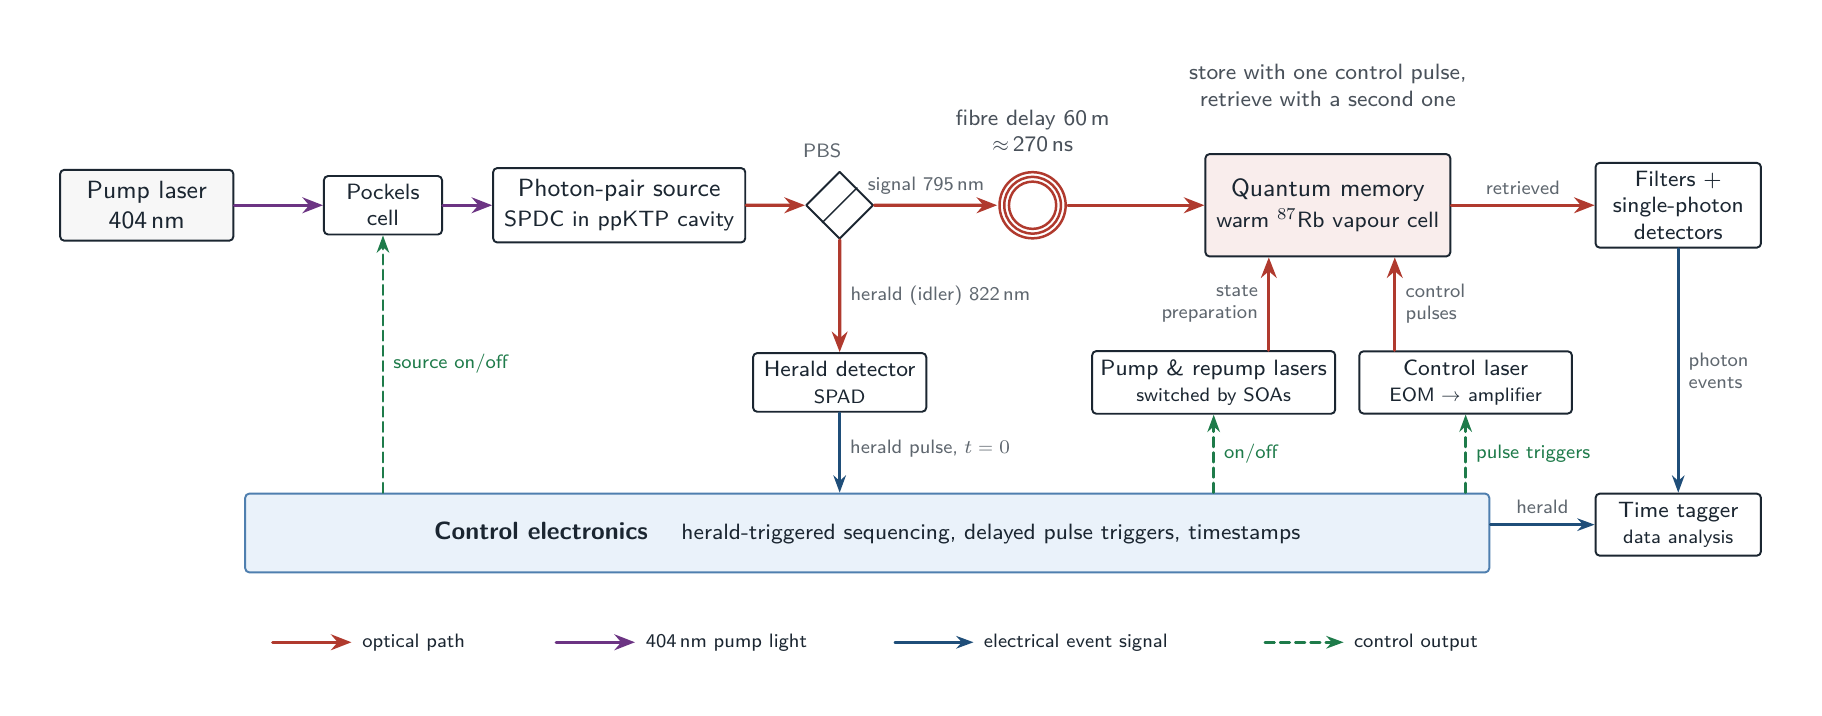
\begin{tikzpicture}[white page, node distance = 6mm]

  % ------------------------------------------------------------ source row
  \node[device, minimum width = 22mm] (pump) at (0, 0) {Pump laser\\\SI{404}{nm}};
  \node[smallblock, minimum width = 15mm] (pc) at (3.0, 0) {Pockels\\cell};
  \node[block, minimum width = 24mm] (spdc) at (6.0, 0) {Photon-pair source\\{\footnotesize SPDC in ppKTP cavity}};
  \node[draw = ink, line width = 0.7pt, fill = white, minimum size = 6mm, rotate = 45,
        inner sep = 0pt] (pbs) at (8.8, 0) {};
  \draw[ink, line width = 0.5pt] (pbs.west) -- (pbs.east);
  \node[tag, above = 2.5mm of pbs] {PBS};

  \draw[pump light] (pump) -- (pc);
  \draw[pump light] (pc) -- (spdc);
  \draw[optical] (spdc) -- (pbs);

  % fibre delay (signal photon)
  \coordinate (coilc) at (11.25, 0);
  \foreach \r in {0.30, 0.36, 0.42} \draw[optical nohead, line width = 0.9pt] (coilc) circle (\r);
  \node[note, above = 5.5mm of coilc] {fibre delay \SI{60}{m}\\$\approx$\,\SI{270}{ns}};
  \draw[optical] (pbs) -- node[above, tag, pos = 0.42] {signal \SI{795}{nm}} ($(coilc) + (-0.45, 0)$);

  \node[block, minimum width = 28mm, minimum height = 13mm, fill = opticallight!45] (mem)
        at (15.0, 0) {Quantum memory\\{\footnotesize warm $^{87}$Rb vapour cell}};
  \draw[optical] ($(coilc) + (0.45, 0)$) -- (mem);

  \node[smallblock, minimum width = 21mm] (det) at (19.45, 0) {Filters +\\single-photon\\detectors};
  \draw[optical] (mem) -- node[above, tag] {retrieved} (det);

  % herald branch
  \node[smallblock, minimum width = 22mm] (spad) at (8.8, -2.25) {Herald detector\\{\scriptsize SPAD}};
  \draw[optical] (pbs) -- node[right, tag, pos = 0.5] {herald (idler) \SI{822}{nm}} (spad);

  % memory drive optics
  \node[smallblock, minimum width = 27mm] (soa) at (13.55, -2.25) {Pump \& repump lasers\\{\scriptsize switched by SOAs}};
  \node[smallblock, minimum width = 27mm] (eom) at (16.75, -2.25) {Control laser\\{\scriptsize EOM $\rightarrow$ amplifier}};
  \draw[optical] (soa.north -| 14.25, 0) -- node[left, tag, align = right] {state\\preparation} (mem.south -| 14.25, 0);
  \draw[optical] (eom.north -| 15.85, 0) -- node[right, tag, align = left] {control\\pulses} (mem.south -| 15.85, 0);

  % ------------------------------------------------------------ electronics
  \node[block, minimum width = 158mm, minimum height = 10mm, fill = syncfill, draw = syncline,
        anchor = north] (ctl) at (9.15, -3.65)
        {\textbf{Control electronics} \quad {\footnotesize herald-triggered sequencing, delayed pulse triggers, timestamps}};

  \draw[elec] (spad.south) -- node[right, tag, pos = 0.45] {herald pulse, $t = 0$} (spad.south |- ctl.north);
  \draw[ctrl] (ctl.north -| pc.south) -- node[right, tag, pos = 0.5, text = ctrl] {source on/off} (pc.south);
  \draw[ctrl] (ctl.north -| soa.south) -- node[right, tag, pos = 0.5, text = ctrl] {on/off} (soa.south);
  \draw[ctrl] (ctl.north -| eom.south) -- node[right, tag, pos = 0.5, text = ctrl] {pulse triggers} (eom.south);
  \node[smallblock, minimum width = 21mm, anchor = north] (tdc) at (19.45, -3.65) {Time tagger\\{\scriptsize data analysis}};
  \draw[elec] (det.south) -- node[right, tag, align = left] {photon\\events} (tdc.north);
  \draw[elec] (ctl.east |- tdc.west) -- node[above, tag] {herald} (tdc.west);

  % ------------------------------------------------------------ captions in figure
  \node[note, anchor = north, text width = 50mm] at ($(mem.north) + (0, 1.25)$)
       {store with one control pulse,\\retrieve with a second one};

  % ------------------------------------------------------------ legend
  \begin{scope}[shift = {(1.6, -5.55)}]
    \draw[optical] (0, 0) -- (1.0, 0) node[right, tag, text = ink] {optical path};
    \draw[pump light] (3.6, 0) -- (4.6, 0) node[right, tag, text = ink] {\SI{404}{nm} pump light};
    \draw[elec] (7.9, 0) -- (8.9, 0) node[right, tag, text = ink] {electrical event signal};
    \draw[ctrl] (12.6, 0) -- (13.6, 0) node[right, tag, text = ink] {control output};
  \end{scope}
\end{tikzpicture}
\end{document}
